\documentclass[main.tex]{subfiles}
\begin{document}
\chapter{Resultate} 

\section{Performance}
Die Tests ergaben eine aufschlussreiche Datenmenge in Hinblick auf die Performance. Dabei sind nicht allein der Durchsatz und die Latenzzeit wichtige Indikatoren. Es gilt ebenfalls zu analysieren, wie die Ressourcen auf der PaaS genutzt wurden. Dabei werden die Daten miteinander verglichen und mögliche Performance-Probleme aufgezeigt. 

% Wie ändert sich das Antwortzeitverhalten in Abhängigkeit von der Last?
% Kann mit dem System auch unter hoher Last noch akzeptabel gearbeitet werden?
% Zeigt das System undefiniertes Verhalten (z. B. Absturz)?
% Geht das System nach Rückgang der Überlast wieder in den normalen Bereich zurück?


\subsection{Durchsatz nach Anfragen}

\subsubsection{Szenario 1 und 2}
Der höchste Durchsatz gelang mit Apache PDFBox (siehe Abbildung \ref{figure:throughputSzen}). Der maximale Durchsatz in der Testreihe betrug 151 Anfragen pro Sekunde. Dies wurde beim Szenario 1 mit der Rate von 50 virtuellen Usern erreicht.  Apache PDFBox hat bei Durchsatz und Verarbeitungsgeschwindigkeit in den ersten beiden Szenarien die höchste Rate im Vergleich zu iText und JasperReports erzielt. 
Der Durchsatz lag beim ersten und zweiten Szenario mit Apache PDFBox bei über 100 Anfragen pro Sekunde, ausser bei den Szenarien 1b und 2b, bei denen die zu verarbeitenden Daten verdreifacht wurden. 
iText zeigt ähnliche Ergebnisse, diesmal mit dem Maximal Durchsatz von 60 Anfragen pro Sekunde im Szenario 2 mit ebenfalls 50 virtuellen Usern. Der Durchsatz von iText und Apache PDFBox schwankt stark. Ein Vergleich vom besten Ergebnis (Szenario 1c) zum schwächsten (Szenario 1b) mit Apache PDFBox zeigt eine Verschlechterung des Durchsatzes von bis zu 60.9\%. Auch bei iText ist eine Verminderung des Durchsatzes festzustellen, die  bis zu 83\% betrug. Hingegen blieb der Durchsatz bei JasperReports vergleichsweise konstant. JasperReports zeigt bei allen Szenarien einen Durchsatz zwischen 11 und und 17 Anfragen pro Sekunde und eine robustere, jedoch langsame Implementierung des Services.
\subsubsection{Szenario 3}
Das dritte Szenario zeigt eine rapide Abnahme der Durchsätze. Alle drei OSREs bringen den Durchsatz nicht über 15 Anfragen pro Sekunde. Das bedeutet, dass im besten Fall das Szenario 3 von JasperReports 52'200 mal in einer Stunde verarbeitet werden kann. iText würde etwa 34'200 PDF in der gleichen Zeit generieren und Apache PDFBox gerade mal 18'360 PDFs liefern. 
Apache PDFBox hat in diesem Szenario die langsamste Verarbeitung mit 1.8 Anfragen pro Sekunde, knapp gefolgt von iText mit 3.1 Anfragen pro Sekunde. 

\begin{figure}[H]
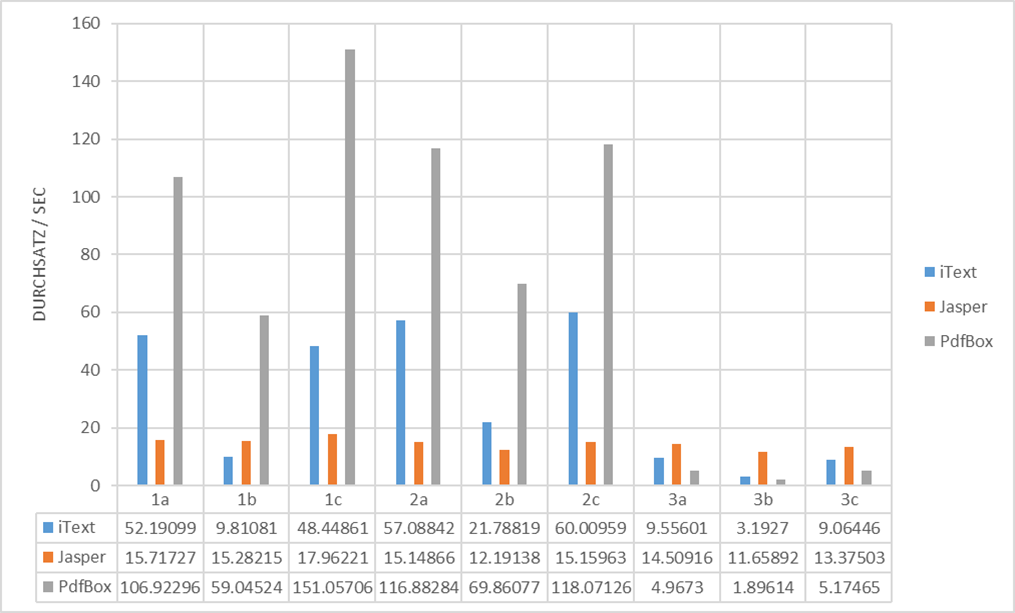
\includegraphics[width=\textwidth]{mainpart/4_analyse_img/VglDurchSzen.png}
 \caption{Vergleich - Durchsatz nach Szenario}
 \label{figure:throughputSzen}
\end{figure}

\subsection{Durchsatz nach Bytes}
Der Durchsatz in Bytes ist über die Testdauer hinweg nicht einbrochen (siehe Abbildung \ref{figure:throughputBytesAll}). Der Durchsatz nach Bytes scheint nur bei JasperReports tief zu bleiben (siehe Zeitschnitt von 03:30:00 bis 06:30:00). Der Durchsatz nach Bytes scheint auch bei Apache PDFBox und iText beim Szenario 3 zu steigen,  wobei der Durchsatz der Antworten nachlässt. Die Analyse der Antworten in Bezug auf Ihre Grösse gibt Hinweise auf dieses Verhalten. 
\begin{figure}[!h]
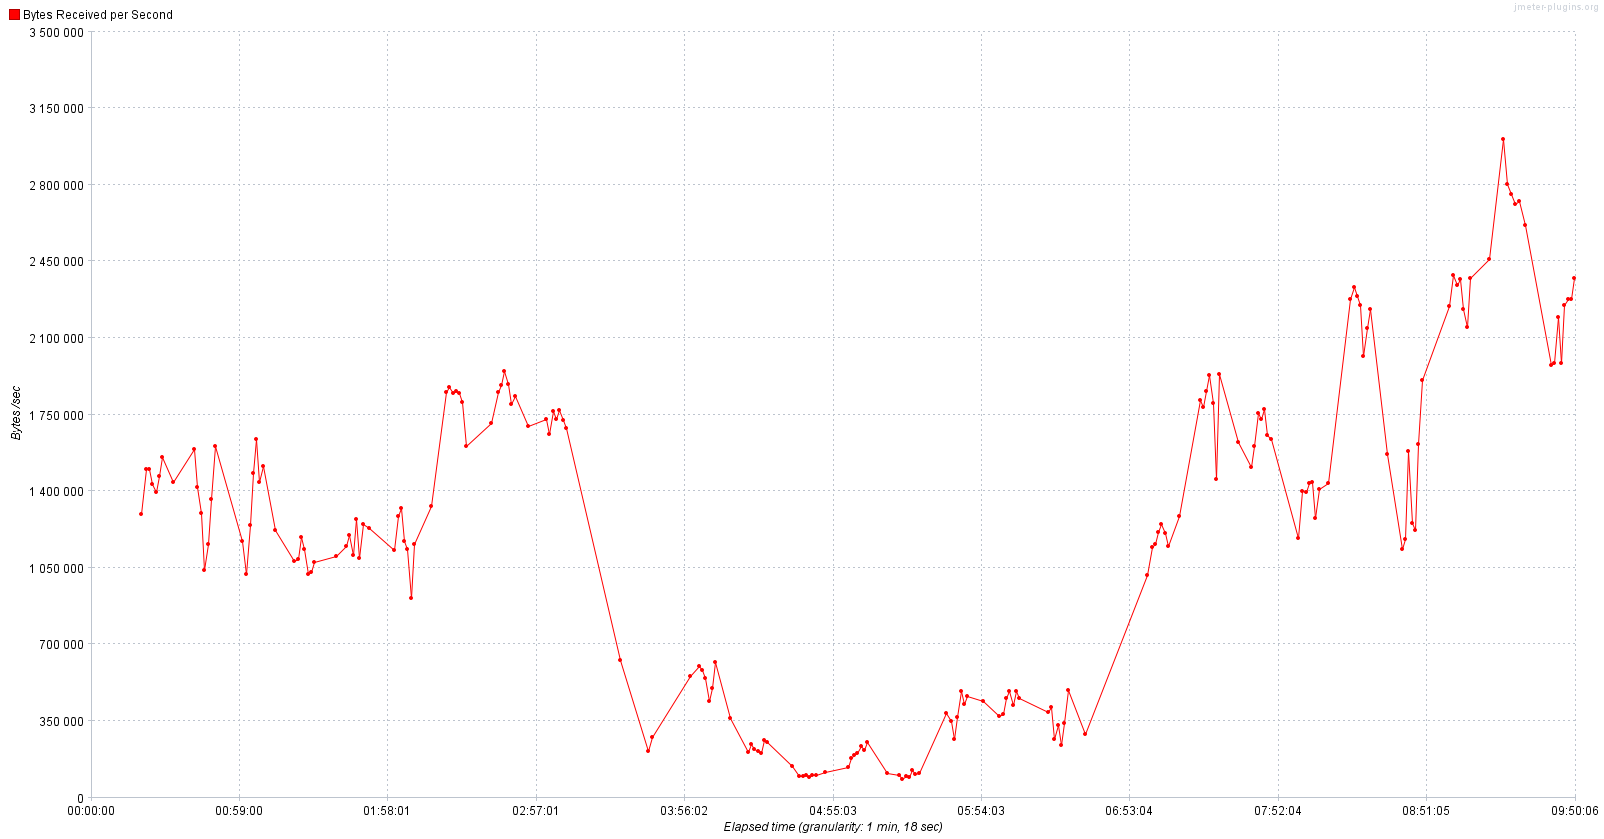
\includegraphics[width=\textwidth]{mainpart/4_analyse_img/ThroughputOverTimeAll.png}
 \caption{Durchsatz in Bytes}
 \label{figure:throughputBytesAll}
\end{figure}


% Diskussion verschoben werden
JasperReports generiert im Vergleich zu den anderen OSREs weitaus kleinere PDFs. Die Kontaktliste, eine Liste mit Kontaktdaten und einem Gender-Symbol, die im Szenario 3 generiert wird, verarbeitet JasperReports besser als die anderen OSREs. JasperReports definiert die Bilder als Typ XObject nur einmal und referenziert dann auf diesen Stream \cite[vgl.~Kap.~5]{whitington_2012}. Dies ist dank der vorkompilierten Templates möglich. Das mit JasperReports generierte PDF ist etwa 46KB gross, das mit Apache PDF-Box generierte PDF ist etwa 730KB gross. Etwas besser ist die Komprimierung bei iText, mit dem das PDF etwa 350 KB gross wird \cite[vgl.~Kap~13]{lowagie_2010}. Dies bedeutet zwar, dass der Durchsatz nicht vergrössert wurde, doch die generierten Files nutzten dennoch die Bandbreite des verfügbaren Netzwerkes. 


\subsection{Latenzzeit}
%Min / Max Average --> Vergleichen mit anderen Projekten wer hat die kürzeste Latenz wer die längste

Die Latenzzeit ist die Zeit, die der Service gebraucht hat, um die Anfrage zu bearbeiten, samt Netzwerkzeit (siehe Abbildung \ref{figure:latencyTestcycle}). 


\begin{figure}[H]
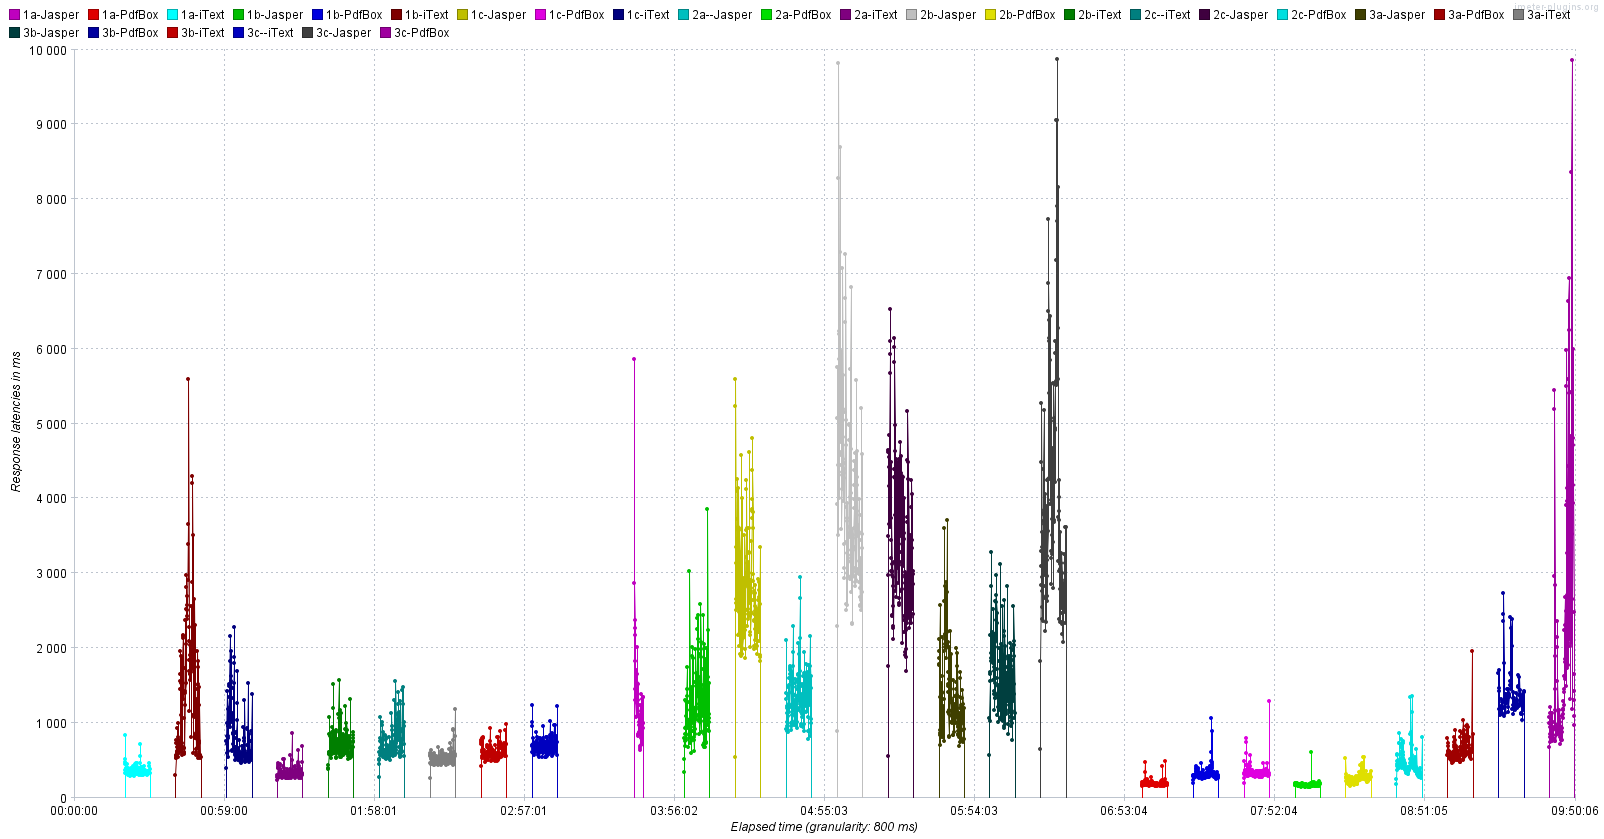
\includegraphics[width=\textwidth]{mainpart/4_analyse_img/ResponseLatenciesOverTime.png}
 \caption{Latenzzeit im Testzyklus}
 \label{figure:latencyTestcycle}
\end{figure}




Auch hier kommen iText und Apache PDFBox bei den meisten Szenarien mit weniger als einer Sekunde aus. Doch es sind auch Ausnahmen festzustellen, wie beim Szenario 1b bei iText und im Szenario 3 bei Apache PDFBox. iText übersteigt im Szenario 1b dabei 4 Sekunden als die Last anstieg. Apache PDFBox zeigt sich über die ersten zwei Szenarien hinweg als schnellstes \acrshort{osre}. Das Szenario 3 zeigt bei allen \acrshort{osre}s eine Anstieg der Latenzzeit. Apache PDFBox hat im Szenario 3a im Durchschnitt noch 3.7 Sekunden und bei Last eine Spitze von etwa 20 Sekunden erreicht. Auch iText zeigt eine rasante Zunahme als das Szenario 3 durchgeführt wurde. Die Spitzen liegen zwischen 12 und 13 Sekunden. JasperReports zeigt eine gewisse Konstanz was die Latenzzeit anbelangt und kann im Szenario 3 noch eine durchschnittliche Latenzzeit unter 8 Sekunden halten (siehe  Abbildung \ref{figure:latencySzenario}).    

% Diskussion
%% Der Serviec ist in den USA ist die Netzwerklatenz so gross um Hunderte oder sogar tausende von Antworten zu stoppen ? 

\begin{figure}[!h]
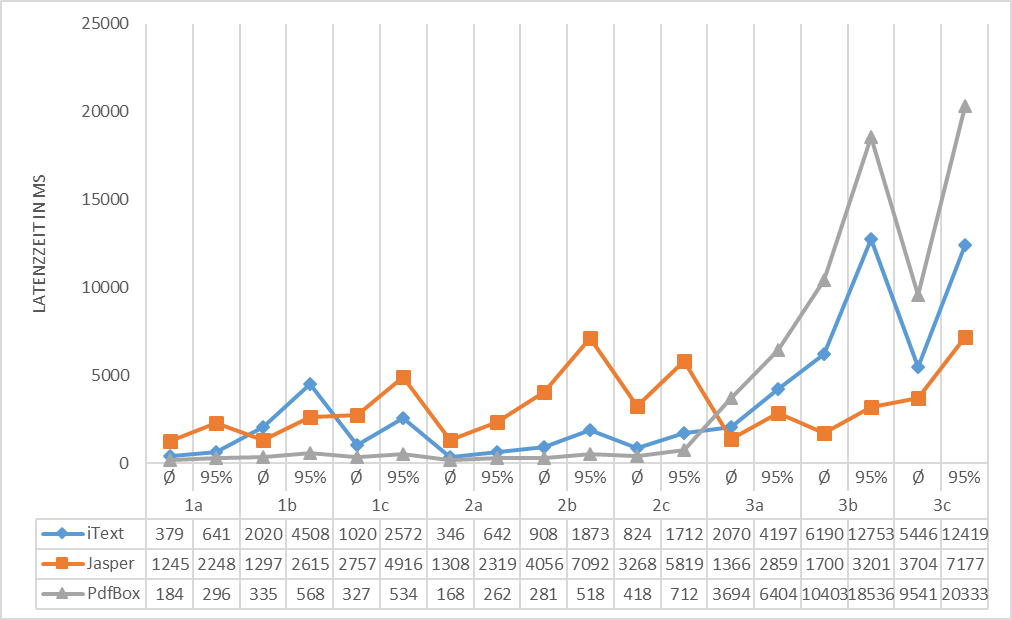
\includegraphics[width=\textwidth]{mainpart/4_analyse_img/LatenzzeitSzen.png}
 \caption{Latenzzeit nach Szenario und OSRE}
 \label{figure:latencySzenario}
\end{figure}

\subsection{Verfügbarkeit}

Der Service soll auch über die Zeit hinweg möglichst verfügbar bleiben. Dies ist ebenfalls ein wichtiger Performance-Indikator. Während der Tests hat keiner der Services über den Testlauf von rund drei Stunden einen Absturz gehabt oder ist unerreichbar gewesen. Die Prototypen waren im Verlauf der Tests meist aktiv geblieben, was aber nicht heisst, dass ein User diese auch als verfügbar empfunden hätte. Hätte man diese Prototypen in einer Produktionsumgebung eingesetzt, wäre der User wohl des Öfteren mit längeren Wartezeiten konfrontiert gewesen. 
Die Latenzzeiten, die im vorhergehenden Kapitel erwähnt wurden, wären auch hier ein Thema. Zum Teil haben eine hohe Anzahl der Anfragen länger als 2 Sekunden gedauert (siehe Abbildung \ref{figure:latencySLA2000}).

\begin{figure}[!h]
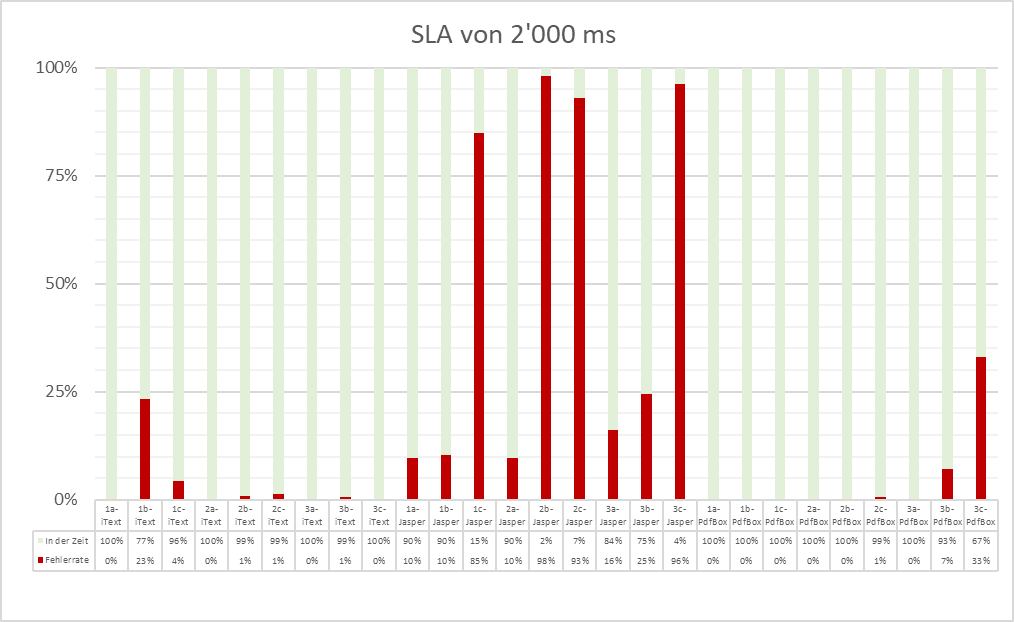
\includegraphics[width=\textwidth]{mainpart/4_analyse_img/latencySLA2000.png}
 \caption{Fehlerrate nach Latenzzeit über 2000ms}
 \label{figure:latencySLA2000}
\end{figure}


% Diskussion  oder Grundlagen?
Nach Miller \cite[Seite~270]{miller_1968} sind Verzögerungen erst dann ein Problem, wenn diese mit dem Fluss der spezifischen Arbeit zusammenkommen. Ein Betriebssystem muss immer in weniger als 0.1 Sekunden antworten, damit es den Arbeitsfluss nicht behindert. Auch hat ein Schreibprogramm in weniger als einer Sekunde zu reagieren, auch wenn Graphiken verarbeitet werden, damit der User in seinem kreativen Prozess nicht behindert wird. Weiter sind die Zeitspannen von 2 bis 4 Sekunden ebenfalls eine wichtige Grösse. Bei komplexen Arbeiten, bei denen der User sich Informationen merken muss, ist es wichtig, diese Antwortzeit so gering wie möglich zu halten.

Besonders JasperReports eignet sich nicht wirlich für eine Online-Applikation (vgl. Abbildung \ref{figure:latencySLA2000}). Vier von neun Szenarien benötigen meist mehr als 2 Sekunden, um eine initiale Antwort zu senden. Die Latenzzeit beträgt bei mehr als 85\% der Antworten mehr als 2 Sekunden. Dies wäre für den Online-Benutzer zu lange, wenn diese Daten für seinen Arbeitsprozess nötig wären.

JasperReports liefert 99\% der Antworten innerhalb von 10 Sekunden, was für eine Batchverarbeitung akzeptabel wäre. Dennoch haben auch iText und Apache PDFBox bei einer \acrshort{sla} von zwei Sekunden in einigen Fällen Schwierigkeiten. iText hat bei der Verarbeitung des Szenarios 1b eine Verfügbarkeit von 77\% erreicht, was zu tief ist für eine Online-Verarbeitung. Bei den übrigen Szenarien, mit der kleinen Ausnahme des Szenarios 1c, das bei 96\% angelangt ist, konnte bei 99\% eine Antwortzeit von unter zwei Sekunden erreicht werden.

Apache PDFBox zeigt hingegen wieder, dass die Verarbeitung der Reports im Szenario 3b und 3c oft eine Geschwindigkeit erreicht, die der User nicht mehr als angenehm oder akzeptabel empfinden würde.








\section{Ressourcen}
Wie bereits erwähnt ist auch wichtig, wie sich der Server während den Test verhält.
Welche Auswirkung die Test auf dem Webservern in Bezug auf Memory und CPU haben, wird in dem folgenden Kapitel behandelt. 

\subsection{Arbeitsspeicher}

Aus den Performance-Messungen konnte der Memory-Verbrauch auf der PaaS geloggt werden (siehe Abbildung \ref{figure:memorytestlauf}). Die Memory-Auslastung steigt bei der Ausführung der Performancetests und sinkt bei der Ausführung des \acrshort{gb} oder einem Neustart des Webservers (Dynos). Die Dynos sind als Standard-X2 definiert, was bedeutet, dass die maximale Auslastung auf den Memory RSS auf 1024MB beschränkt ist \cite[vgl.~Kap~7.7]{hanjura_2014}. Dies bedeutet, dass die Auslastung auf dem Memory begrenzt ist und jede weitere Verarbeitung auf den SWAP ausgelagert wird (siehe Abbildung \ref{figure:memorytestlauf}). iText nutzte nur wenig SWAP und konnte in den Performancetests mit RSS Memory meist alle Anfragen bearbeiten. Ein Teil der Anfragen wurde dennoch im Szenario 3 im SWAP ausgelagert. Nach einem Restart des Webservices wurde JasperReports genutzt. Diese ORSE nutzte bereits das verfügbare Memory im ersten Szenario. Das Memory auf dem SWAP konnte über alle Szenarien hinweg nicht freigegeben werden, was zu einem Aufblasen des Memory-Verbrauchs führte. JasperReports erreichte im Testlauf einen totalen Memory-Verbrauch von 1389.32MB. Apache PDFBox erreichte im Testlauf die Memory-Quota von 1024 MB kaum.




\begin{figure}[H]
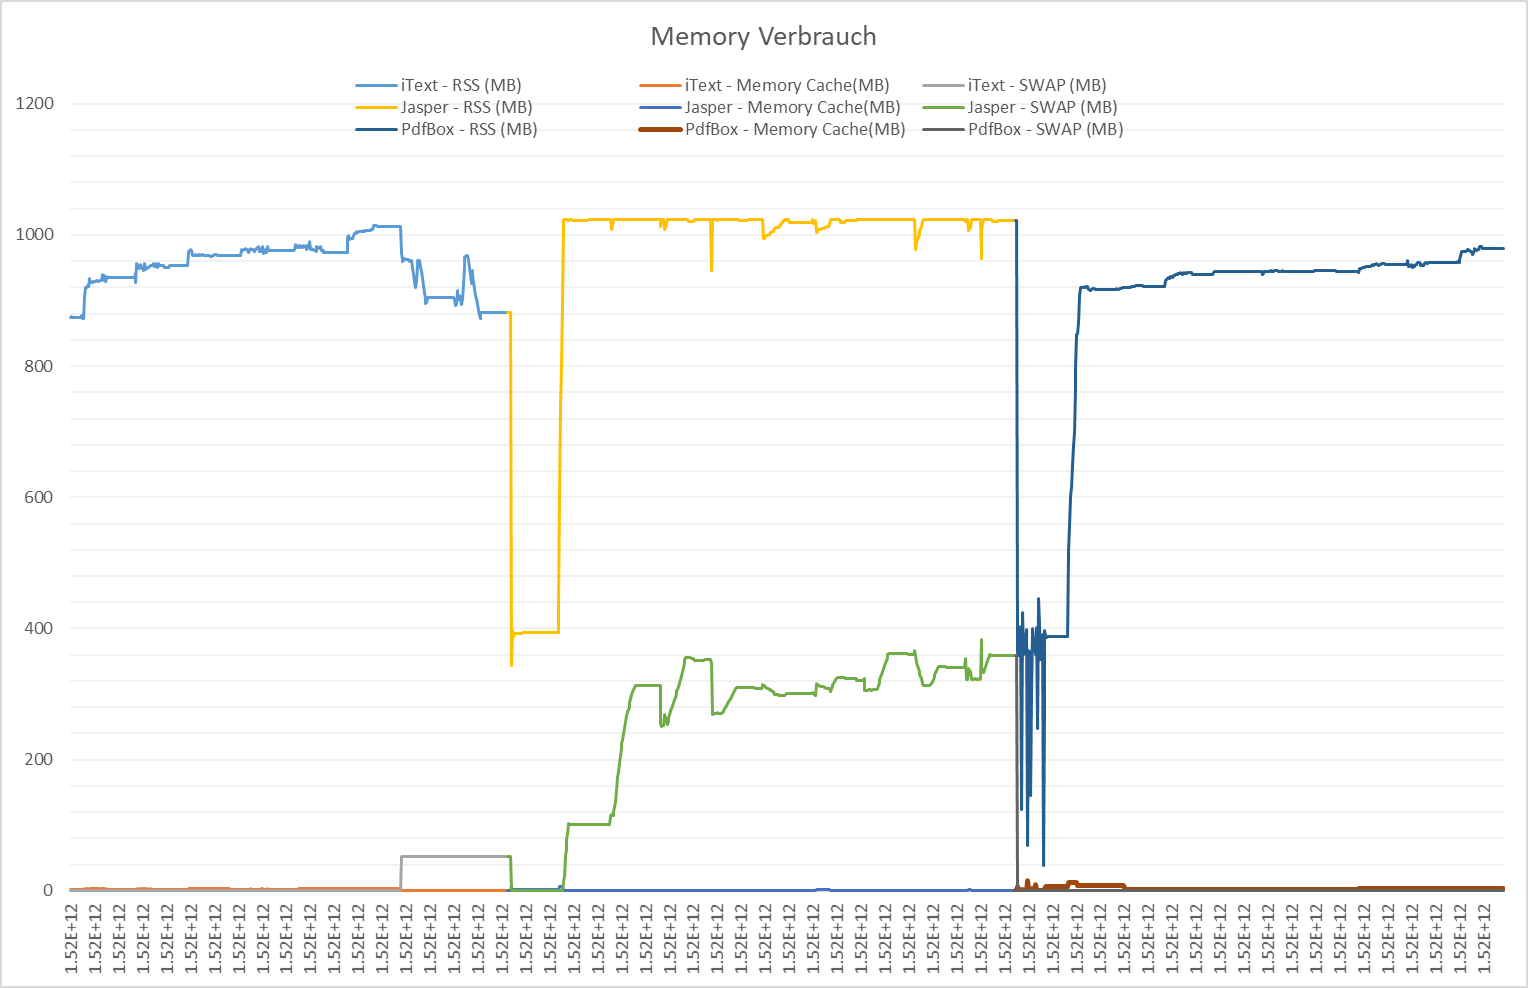
\includegraphics[width=\textwidth]{mainpart/4_analyse_img/MemoryVerbrauch.png}
 \caption{Memory-Verbrauch Testlauf}
 \label{figure:memorytestlauf}
\end{figure}



\subsection{Prozessor Last}

Der Verbrauch des CPU ist eine etwas schwierige Messgrösse. Die \acrshort{paas} hat diese Daten mit der Stichprobengrösse von einer Minute in die Logdateien geschrieben.

Dabei ist zu erkennen, dass sich im Testzyklus von iText  die Auslastung je nach Szenario sehr stark unterscheidet. Z.B. sind während des zweiten Szenarios durchschnittlich zwischen vier und sieben Prozesse im Status 'Ready' pendent gewesen. Hingegen sind im dritten Szenario fast immer alle Prozesse in Ausführung gewesen, das bedeutet eine fast optimale Auslastung des CPUs mit wenigen wartenden Prozesse. Diese sind wohl so entstanden, da die Prozesse im dritten Szenario langläufiger waren und somit wenig neue Anfragen verarbeitet wurden (siehe Abbildung \ref{figure:cpuVergleich}).

JasperReports hat den CPU eher gefordert und hat über den ganzen Zeitraum viele Prozesse gebraucht. Wie intensiv die Verarbeitung von JasperReports im Vergleich zu den anderen OSREs ist, wird hier hervorgehoben. Apache PDFBox ist hier als sehr sparsam zu erkennen. Es wurden maximal etwa 
fünf Prozesse ausgelagert. 
\begin{figure}[H]
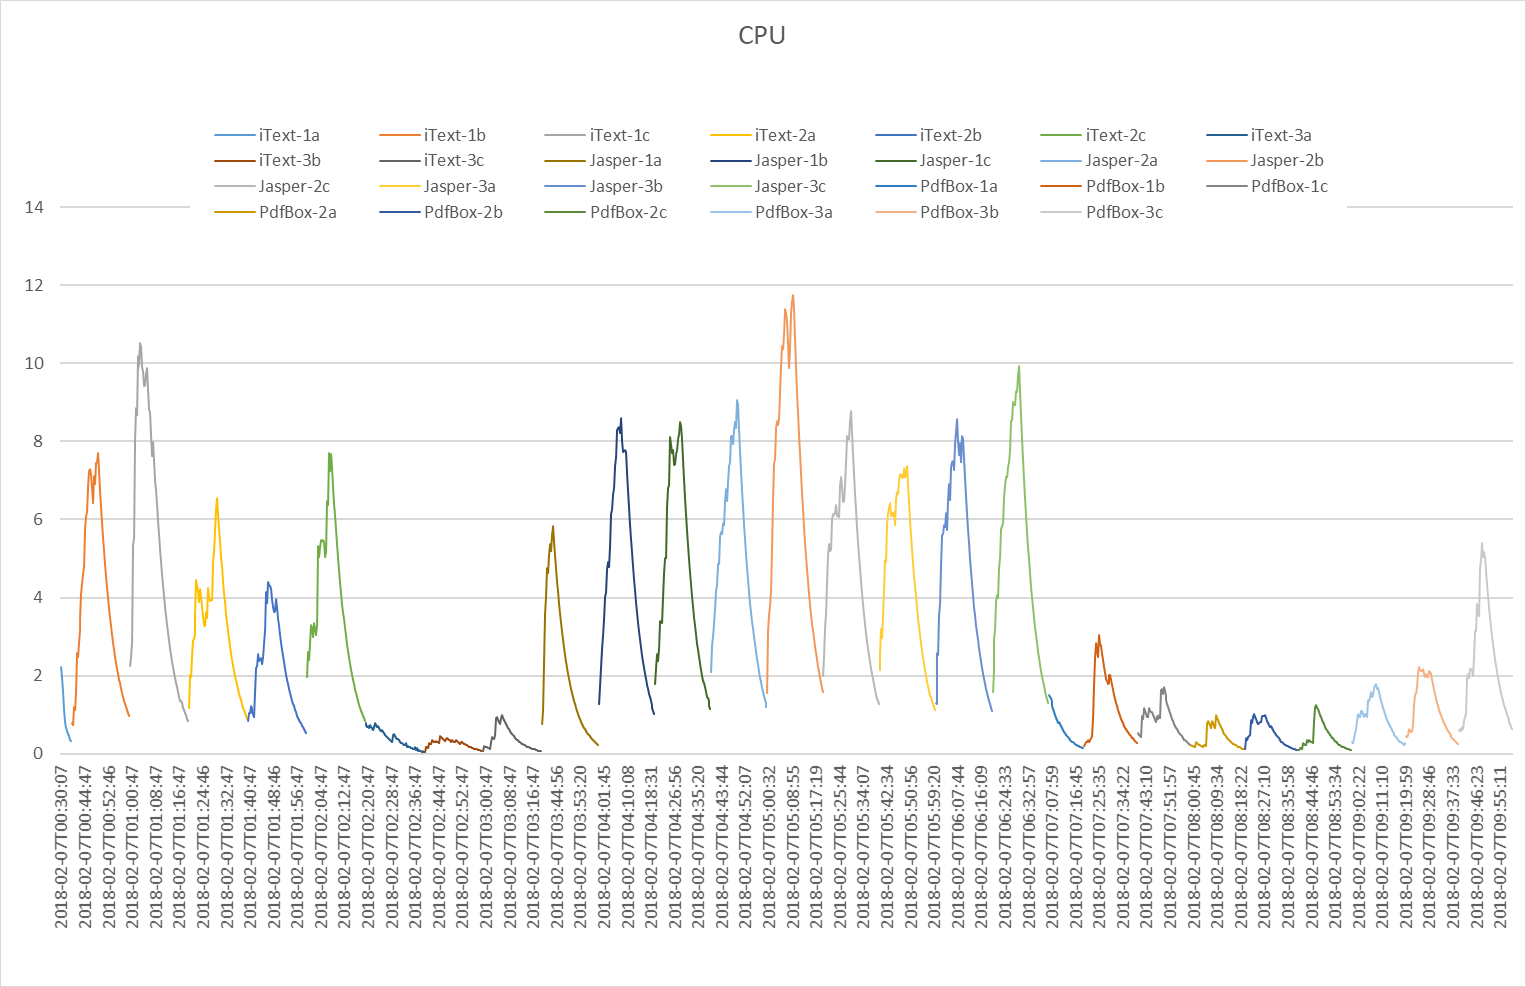
\includegraphics[width=\textwidth]{mainpart/4_analyse_img/CPUVergleich.png}
 \caption{Vergleich - CPU-Last nach Szenario}
 \label{figure:cpuVergleich}
\end{figure}


\section{Lastveränderung}

Die OSREs haben sich während des Tests in Bezug auf die Lastveränderung verschieden verhalten. In diesem Kapitel sollen die Veränderungen von Requestgrössen und die Zunahme von virtuellen Usern (\acrshort{vu}) weiter aufgezeigt werden.


\subsection{Requestgrösse}
Im Vergleich zu den Szenarien 1a, 2a und 3a wurden bei den Szenarien 1b, 2b und 3b die Datensätze für die Verarbeitung verdreifacht, was dazu geführt hat, dass sich alle Antwortzeiten und Durchsätze verschlechtert haben (vgl. Abbildungen \ref{figure:vglABRequ}).

\begin{figure}[H]
\centering
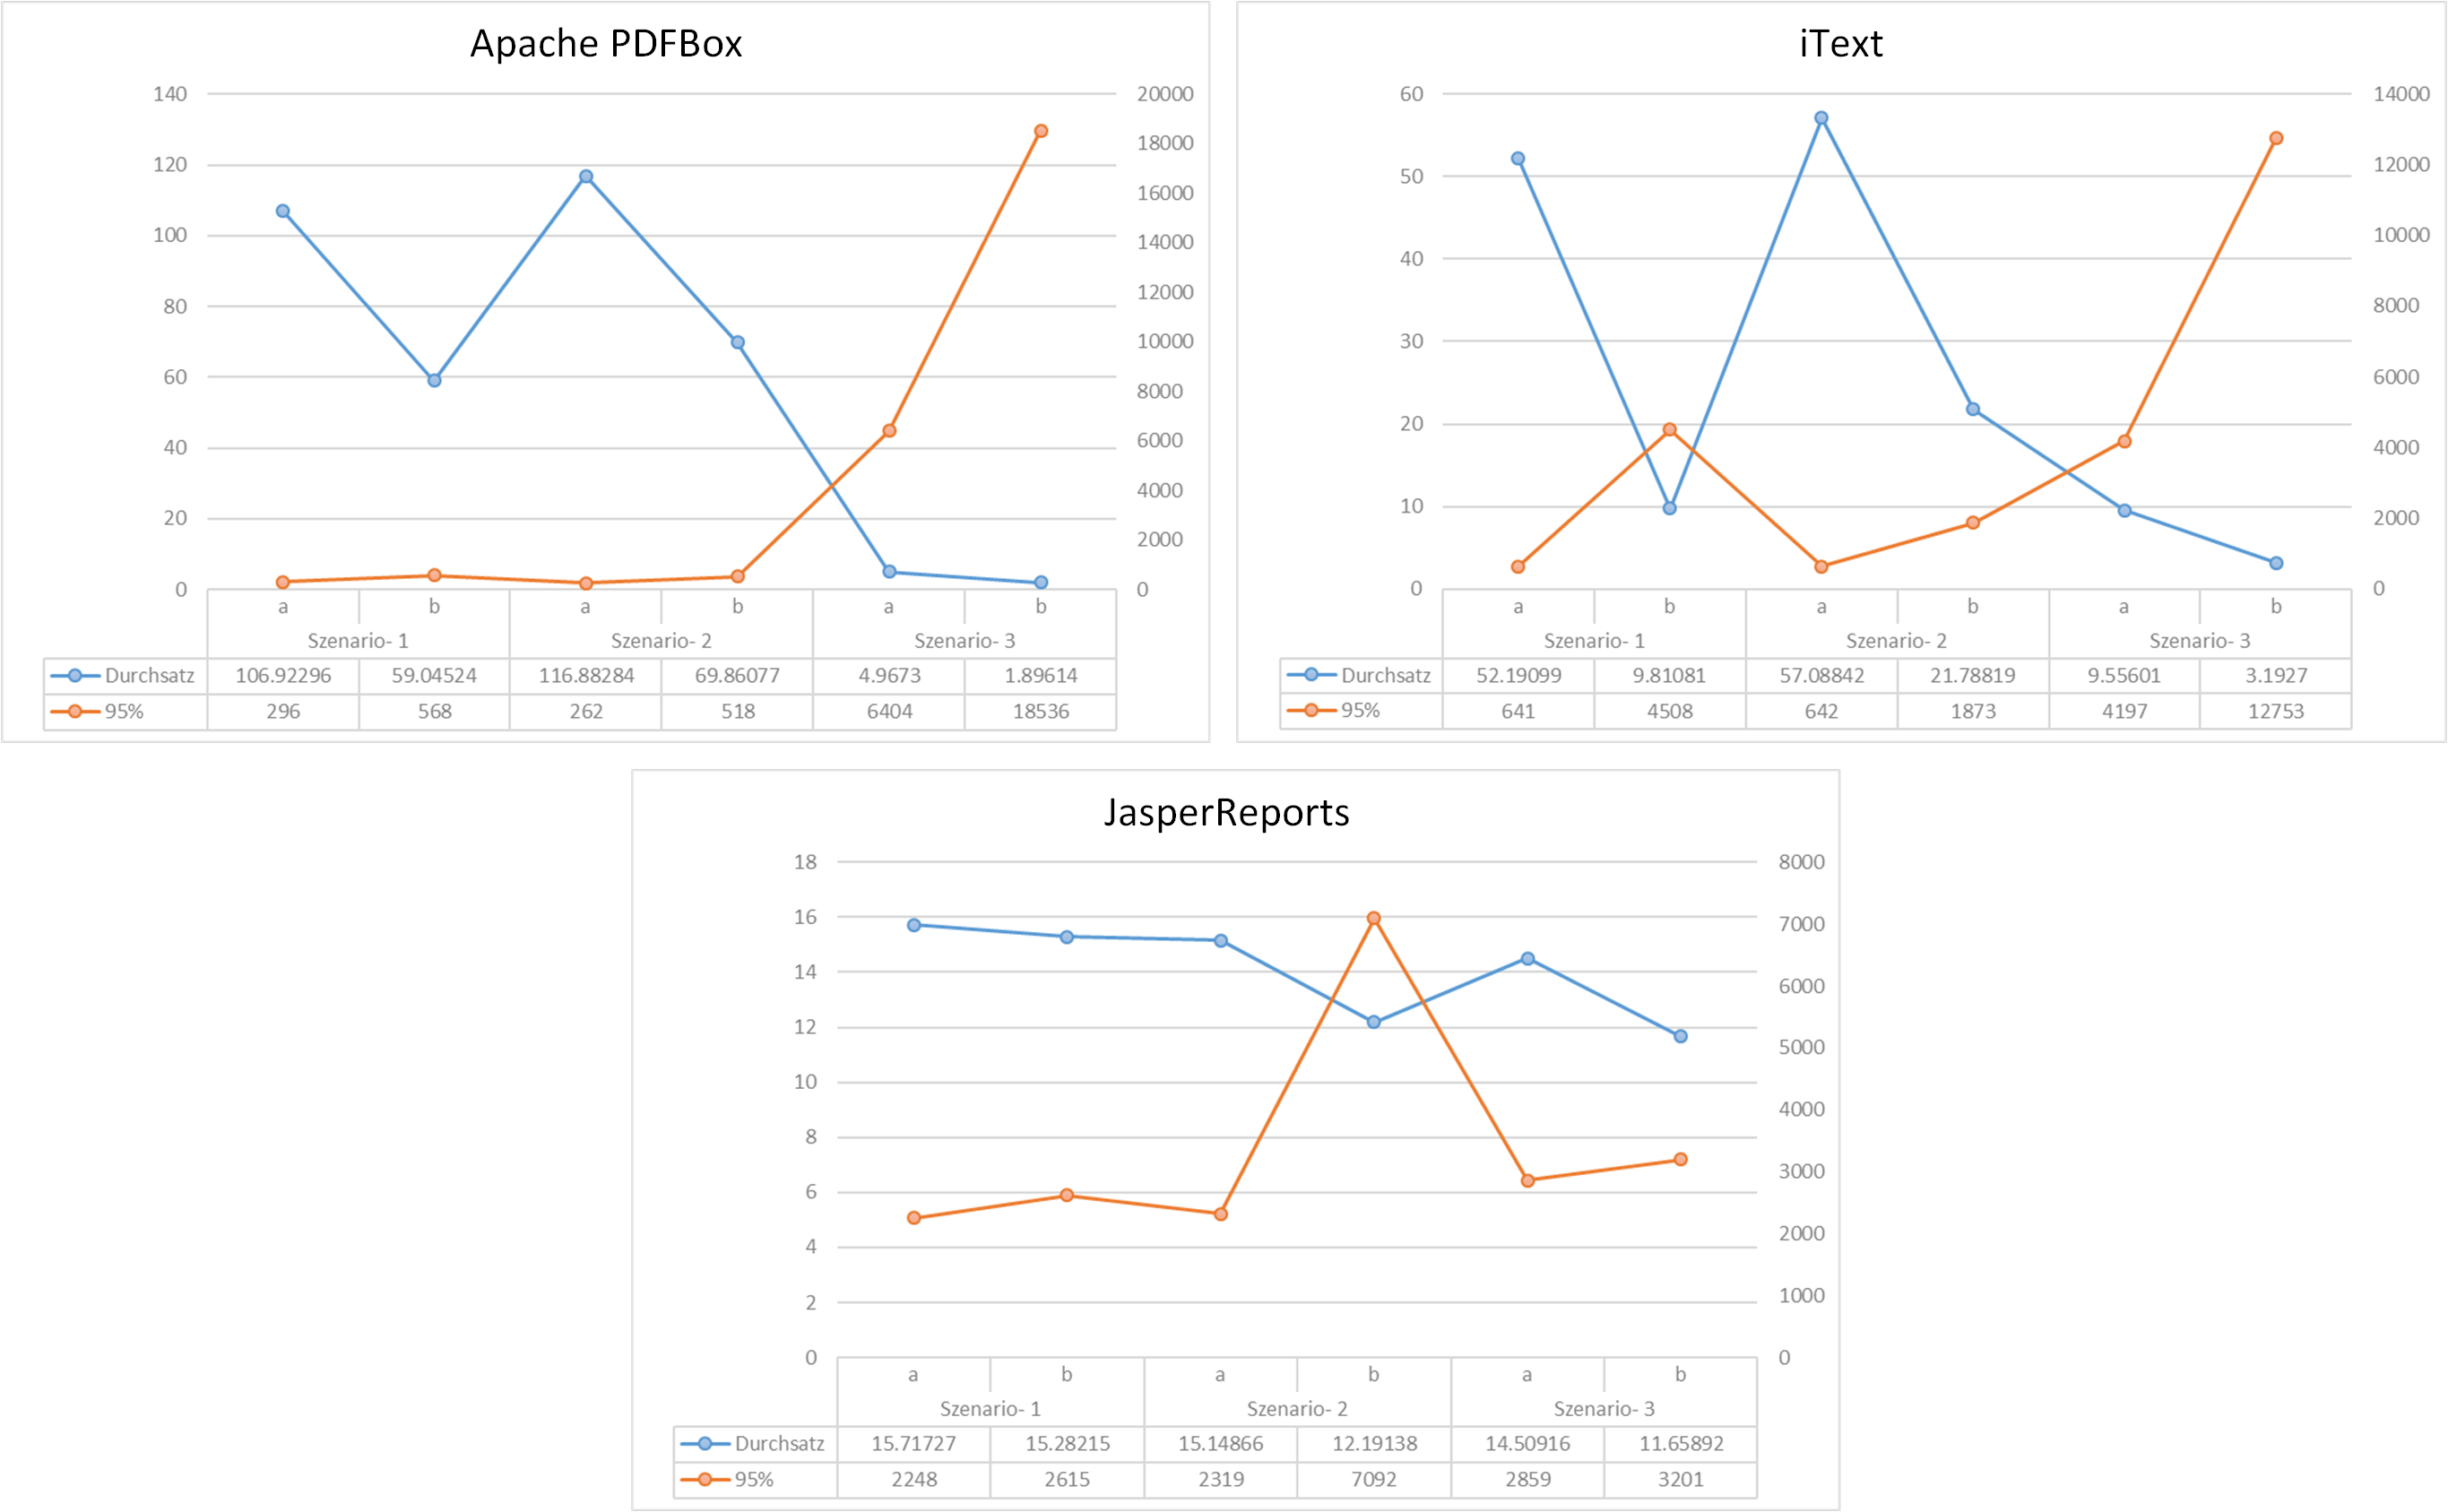
\includegraphics[width=0.7\textwidth]{mainpart/4_analyse_img/ABAuswertung.png}
 \caption{Vergleich Baseline mit grösserer Datenmengen}
 \label{figure:vglABRequ}
\end{figure}


Der Durchsatz von Apache PDFBox verschlechtert sich im ersten Szenario von 106.92 auf 59.04 Anfragen pro Sekunde was ein Rückgang von 44\% bedeutet und etwa gleich sieht es auch im zweiten Szenario aus. Bei diesem ging der Durchsatz ebenfalls um 40\% zurück. Im Szenario 3 sind die Durchsätze ebenfalls zurück. Zwar waren diese bereits sehr tief, doch gingen ebenfalls um etwa 3 Anfragen pro Sekunde zurück, was etwa 62\% Rückgang bedeutet. 


iText verzeichnet hier ebenfalls Durchsatzeinbrüche, wie es in den ersten zwei Szenarien zu sehen ist. Bei beiden Szenarien fällt der Durchsatz je von 52 auf 9.8 und von 57 auf 21 Anfragen pro Sekunde. Was bedeutet, dass der Durchsatz bei iText um 81\% beim ersten und 63\% beim zweiten Szenario fällt.
Auch im dritten Szenario fällt der Durchsatz. Es sind ebenfalls zwei drittel weniger Anfragen pro Sekunde möglich. 

JasperReports hat sich etwas stabiler verhalten. Der Durchsatz ist in allen drei Szenarien gesunken, doch zum Teil nur minim. Der erste Szenario hat knapp 0.44 Anfrage pro Sekunde weniger verarbeitet verglichen mit dem Szenario 1a. Das ist eine Verschlechterung des Durchsatzes von 2.8\%. Der zweite und dritte Szenario sanken um je 19.5\%.  

Hier sei noch einmal hervorgehoben, dass diese Daten aufgrund eines Testlaufs ermittelt wurden. Es kann in jedem Testlauf das gleiche Phänomen beobachtet werden, dennoch sind diese Daten nicht stellvertretend oder absolut zu betrachten. Grössere Ausreisser wurden in anderen Testläufen ebenfalls aufgezeichnet.

Die Latenzzeiten sind bei allen gestiegen. Wir vergleichen hier mittels dem 95\% Perzentil, was bedeutet, wir vergleichen, welche Zeiten 95\% der User gespürt hätten. Dabei hätten 5\% längere Antwortzeiten gehabt und die restlichen 95\% die angegebene Zeit oder weniger.

Apache PDFBox hat bei den beiden ersten Szenarien eine Latenzzeit von 296 und 262. Beim Steigen der Last sind diese dann auf 568 und 518 gestiegen. Die meisten Users hätten diese Verzögerung nur leicht gemerkt. Beim Szenario 3 sind diese Zeiten von bereits 4.9 Sekunden auf 18.9 Sekunden gestiegen. 5\% der User hätten dabei noch länger warten müssen, um eine Antwort zu erhalten. 

iText hat bei diesen Requestgrössen gleich sieben Mal länger gebraucht, um eine Antwort zu liefern. Die Latenzzeit stieg beim 95-Perzentil von 641 auf 4508. Ähnlich, aber nicht ganz so schlimm ist im Szenario 2 zu sehen, da steigt die Latenzzeit von 642 auf 1873, was drei Mal länger dauerte. Das erste Szenario stösst dabei an die Geduldsgrenze der meisten User.  Szenario 2 liegt dabei mit 1.8 Sekunden noch im Rahmen, um den Arbeitsfluss eines Users nicht zu unterbrechen. Im dritten Szenario ist wie bei Apache PDFBox eine deutliche Abnahme der Reaktionszeit zu sehen. Die Latenzzeit steig dabei von 4.1 auf 12.8 Sekunden. 

Die Latenzzeit von JasperReports bleibt bei dem ersten und dem dritten Szenario zwischen 2 und 3 Sekunden. Das Szenario 2 ist hat dabei einen Anstieg von 2.3 auf 7 Sekunden . Die CPU-Last steigt auch dort höher als bei den anderen Szenarien (siehe Abbildung \ref{figure:cpuVergleich}). 


\subsection{Virtuelle User}
Die Prototypen wurden während den Test von den initialen 20 \acrshort{vu} im Szenario 'a' weiter gefordert, als 30 weitere \acrshort{vu}s hinzugefügt wurden, um eine erhöhte Nutzerinteraktion zu simulieren. Wie die \acrshort{osre} dabei reagiert haben (siehe Abbildungen  \ref{figure:vglACVU}). In den Diagrammen werden die Veränderungen des Durchsatzes mit dem  95-Perzentil der Antwortzeit verglichen.


Einige der Erkenntnisse in diesem Zusammenhang können bei Apache PDF-Box gesehen werden. Als die Nutzerlast stieg, stieg auch der Durchsatz im Szenario 1 von 106 auf 151 Anfragen pro Sekunde. Die Antwortzeit verdoppelte sich dabei. Ähnliches ist auch im zweiten Szenario zu beobachten. Apache PDFBox hat Mühe mit dem Szenario 3. Die Antwortzeit verdreifacht sich dabei, wobei der Durchsatz gleich bleibt.

iText scheint in der Implementation der ersten zwei Szenarien ein ähnliches Verhalten unter Last zu erzeugen. Die Antwortzeit wird im ersten Szenario viermal langsamer, im Szenario 2 dreimal langsamer. Auch iText schafft es, seinen Durchsatz zu verbessern, und zwar werden drei Antworten mehr pro Sekunde verarbeitet. Szenario 3 hat ähnliche Probleme wie Apache PDFBox. Die Antwortzeiten verdreifachen sich und der Durchsatz bleibt auch bei iText etwa konstant.

JasperReports verschlechtert sich in allen Antwortzeiten, aber nicht ganz so extrem wie iText und Apache PDFBox. In allen Szenarien verschlechtern sich die Antwortzeiten. Bei allen Szenarien wurde JasperReports etwa doppelt so langsam. Was den Durchsatz anbelangt, blieb dieser fast konstant. Im Szenario 1 wurde dieser ebenfalls etwas höher (2 Anfragen pro Sekunde mehr).


\begin{figure}[H]
\centering
\includegraphics[width=0.7\textwidth]{mainpart/4_analyse_img/ACAuswertung.png}
 \caption{Vergleich Baseline mit mehr \acrshort{vu}}
 \label{figure:vglACVU}
\end{figure}


\end{document}